\section{はじめに}

本書は初めて領域気象気候モデル (SCALE-RM)を利用するユーザー向けに解説したユーザーズガイドです。
本書はSCALE-RM version \version に対応した説明になっています。
第\ref{sec:overview}章でSCALEの概要について説明し、
第\ref{sec:install}章で必要な環境、およびインストール方法を説明します。
%
続いて、第\ref{sec:tuto_ideal}章では理想実験、
第\ref{sec:tuto_real}章では現実大気実験の実行方法について
簡単な例示しながら説明します。
第\ref{sec:install}章から第\ref{sec:tuto_real}章まではひと繋がりの
チュートリアルとなっており、前章の経験や結果に基づいて説明する部分がありますのでご注意下さい。
%
第\ref{sec:advance}章では、チュートリアルを終えたユーザー向けに
設定の変更、機能やツールについて説明します。

本書中の不明点やお気づきの点がございましたら、SCALE user's メーリングリスト\\
 \verb|scale-user@riken.jp|までご連絡ください。



\subsection{SCALEの特徴}
SCALE(Scalable Computing for Advanced Library and Environment)は
計算機を用いて気象・気候科学の問題にアプローチする際に、
ユーザーが研究を進めやすいように、
事前処理から数値計算、解析に至るまですべての過程を網羅する数値計算ライブラリを
目指したソフトウェアであり、下記に挙げるような特徴を持つ。
\begin{itemize}
\item SCALEは、「BSD-2ライセンス」のもとでオープンソースソフトウェア
として提供されており、商用、非商用に関わらず自由な利用・改変・再配布が可能である。
\item SCALEには、SCALE-RM(SCALE-Regional Model)、SCALE-GM(SCALE-Global Model)といった組み上げ済みの数値モデルが含まれている。
\item SCALEには、次節で説明する様々なコンポーネントが導入されており、
必要に応じて取り替えることが可能である。
\end{itemize}

ライセンスの詳細は、トップディレクトリ直下の``\verb|scale/LICENSE|''のファイルに記述されている。
SCALEの使用前に一読しておくこと。またSCALEのWebページにも説明が記載されているので必要に応じて
参照すること(\url{http://scale.aics.riken.jp/})。

\subsection{SCALE-RMモデルの構成}
現在、SCALEには下記のコンポーネントが実装されている。
SCALE-RM からはすべてのコンポーネントが利用可能である。
詳細なモデル構成や差分化手法については、
\citet{scale_2015}、\citet{satoy_2015b}、および\citet{nishizawa_2015}を参照されたい。\\


\noindent{\bf フレームワーク関係}
\begin{itemize}
 \item カーテシアン(Cartesian)グリッドシステム(Arakawa C-grid)
 \item MPI通信を用いた二次元領域分割
 \item Map-projection \& Map-factors
 \item Nesting システム(1-way:親→子のみ)
   \begin{itemize}
    \item Option: オンライン実行(複数ドメインの計算を同時に実行)とオフライン実行(外側ドメインの計算終了後に、その結果を用いて内側ドメインの計算を行う)を選択可能
   \end{itemize}
 \item 複数事例一括実行 システム(バルクジョブシステム)
 \item gtoolベースnetcdf4ファイル I/O
 \item 外部データ読み込みによる初期値・境界値データ作成
   \begin{itemize}
    \item Option: WRF-ARW、NICAM、その他GrADSフォーマットでの入力に対応
   \end{itemize}
\end{itemize}

{\bf 力学コア関係}
\begin{itemize}
 \item 方程式系: 3次元完全圧縮非静力学方程式系
 \item 数値解法: 陽解法と陰解法の両方を実装
   \begin{itemize}
    \item Option: HE-VE(陽解法)
    \item Option: HE-VI(水平方向は陽解法-鉛直方向は陰解法)
%    \item Option: HI-VI(陰解法)
   \end{itemize}
 \item 空間差分:
    \begin{itemize}
      \item 2次中央差分(2-nd order central difference schemes)
      \item 4次中央差分(4-th order central difference schemes)
      \item 6次中央差分(6-th order central difference schemes)
      \item 3次風上差分(3-rd order upwind difference schemes)
%      \item 3次風上差分(Koren(1993)filterあり)(3rd order upwind difference scheme with \citet{Koren_1993} filter)
      \item 5次風上差分(5-th order upwind difference schemes)
    \end{itemize}
 \item 時間差分:
    \begin{itemize}
      \item 3次ルンゲクッタスキーム(Heun's 3rd order Runge-Kutta scheme)
      \item Wicker and Skamarock (2002) 3段ルンゲクッタスキーム \citep[3-step Runge-Kutta scheme of ][]{Wicker_2002}
      \item 4次ルンゲクッタスキーム(4th order Runge-Kutta scheme)
    \end{itemize}
 \item 非負保証:
    \begin{itemize}
      \item フラックス修正法(Flux Corrected Transport)
      \item Koren (1993) filter \citep{Koren_1993} (3次風上差分スキーム使用時のみ)
    \end{itemize}
 \item 数値フィルター: 4次超粘性(4-th Hyper diffusion)
 \item 地形: Terrain following coordinate(地形に沿った座標系)
\end{itemize}


{\bf 物理過程}
\begin{itemize}
 \item 乱流過程: 複数から選択可能
   \begin{itemize}
    \item Smagorinsky-Lilly typeのサブグリッドモデル \citep{smagorinsky_1963,lilly_1962}
    \item Deardorff(1980) サブグリットモデル \citep{Deardorff_1980}
    \item MYNN2.5境界層モデル \citep{my_1982,nakanishi_2004}
   \end{itemize}
 \item 雲微物理: 複数から選択可能
   \begin{itemize}
    \item Kessler type バルクモデル \citep{kessler_1969}
    \item 6-class single moment バルクモデル \citep{tomita_2008}
    \item 6-class double moment バルクモデル \citep{sn_2014}
    \item ビン法雲モデル \citep{suzuki_etal_2010}
   \end{itemize}
 \item 放射過程: MSTRN-X \citep{sekiguchi_2008}
 \item 地表面モデル
  \begin{itemize}
   \item 陸面モデル: バケツモデル \citep[バルク交換係数は][]{beljaars_1991,wilson_2001}
   \item 海洋モデル:(スラブモデル)
   \item 都市モデル: 単層キャノピーモデル \citep{kusaka_2001}
  \end{itemize}
\end{itemize}

上記に加え、SCALE-RM のコンポーネントとして、
現実事例の計算に必要な地形や土地利用データを作成するツール、
理想実験の初期値・境界値、もしくは外部モデルから初期値・境界値を作成するツールが提供されている。

次節でSCALEの思想とモデルの関係について説明するが、
SCALE-RMの実行とは直接関係ないため、
必要なければ読み飛ばしても構わない。


\subsection{SCALEのライブラリとモデル}

\begin{figure}[bh]
\begin{center}
  
\includegraphics[width=0.9\hsize]{./figure/library.eps}\\
  \caption{SCALEのねらい}
  \label{fig:scale}
\end{center}
\end{figure}

SCALEは、理化学研究所 計算科学研究機構(RIKEN AICS)を中心に
開発が進められている気象・気候科学計算向けのライブラリである。
図 \ref{fig:scale}にSCALEの思想の概念図を示す。
この図に示されるように、SCALEは、近い将来もしくは
現在すでに研究の足かせとなっている諸問題を解決する、もしくは解決の手助けをすることを目指している。
SCALEは次世代のスーパーコンピュータから小型PCクラスターに至るまで
広く用いられる事を念頭において開発されており、
気候・気象科学を専門とする科学者と計算機科学を専門とする科学者が共同で開発を行っている。
そのため、スーパーコンピュータ「京」やFujitsu FX10等のスーパーコンピュータ上でも、
高い計算効率がでるように設計されている。
ユーザーには、スーパーコンピュータ「京」を
はじめとする並列計算機に対してチューニングされた
モデルコンポーネントや解析システム、テストセット、
そして「開発環境」を提供する。

SCALEを利用した数値モデルとして、
SCALE-RMが含まれている(図 \ref{fig:scale-rm})。
格子系、力学コア、各種物理過程などの基本的なコンポーネントは
SCALEが提供する。
SCALE-RM は、予報変数などをコンテナを持ち、
SCALEのコンポーネントを適切に呼び出すことで時間発展計算を行っている。
ユーザーは、必要に応じて、各コンポーネントを選択し、組み合わせて使用することが可能である。
このSCALE-RMを気象研究に適用した事例には
\citet{satoy_2014}、\citet{satoy_2015}がある。
ユーザーは、SCALEを用いてSCALE-RMと同様な方法によって
新たなモデル作ることができる。


\begin{figure}[tb]
\begin{center}
  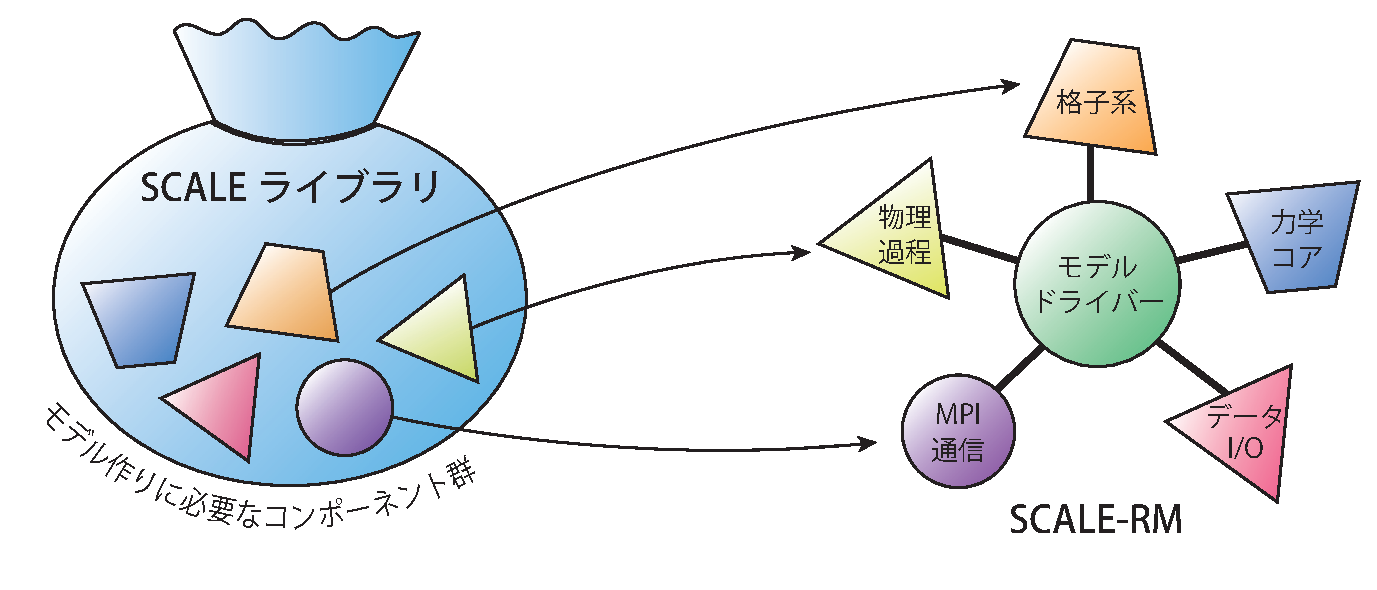
\includegraphics[width=0.9\hsize]{./figure/scale.eps}\\
  \caption{SCALEとSCALE-RMの関係}
  \label{fig:scale-rm}
\end{center}
\end{figure}


\section{表記上の注意}

本書中では、Unix での bash 上での実行を想定して記述している。
異なる環境下では適宜読み替えて対応すること。
また、本書内では特に断りがない限り、下記の表記法に従うものとする。


コマンドラインのシンボル(\verb|$, #|)は、コマンドの実行を示す。
下記の表記の違いは、プログラムを実行する権限の違いを示している。

\begin{verbatim}
 #        <- root権限で実行するコマンド
 $        <- ユーザ権限で実行するコマンド
\end{verbatim}
権限の一時的な切り替えにはsuコマンドを用いる。
\verb|{User_Name}|は実際のユーザ名に読み替えること。
\begin{verbatim}
 $ su {User_Name}   <- {User_Name}のユーザー名でログイン
 $ exit             <- {User_Name}のユーザー名でログインを終了
 $ su -             <- root権限に変更
 #
\end{verbatim}

コマンドオプションにハイフンを用いると、そのユーザでのログインを行う。
用いない場合、権限のみの変更となる。またユーザ名を省略するとrootでのログインを試す。
ユーザの一時切り替えを終わるには、exitコマンドを用いる。
%各プログラムをインストールするための圧縮ファイルは、/tmpにダウンロードされていると仮定する。
%他のディレクトリにダウンロードしてある場合は、mvコマンド等を用いて/tmpに移動しておくことを勧める。
文章表記のうち、ダブルスラッシュ(//)で始まる行は解説のためのもので、実際に記述する必要はない。

下記のように四角い囲みで区切られた部分は、コマンドラインのメッセージ部分を表す。\\

\noindent {\small {\gt
\fbox{
\begin{tabularx}{140mm}{l}
 -- -- -- -- コマンドラインのメッセージ\\
 -- -- -- -- -- -- -- -- コマンドラインのメッセージ\\
 -- -- -- -- -- -- -- -- -- -- -- -- コマンドラインのメッセージ\\
\end{tabularx}
}}}\\

また、下記のように丸い囲みで区切られた部分は、エディタでファイルを編集する記述内容を表す、
もしくはファイル内の記述を参照している部分である。\\

\noindent {\small {\gt
\ovalbox{
\begin{tabularx}{140mm}{l}
 -- -- -- -- ファイル中の記述\\
 -- -- -- -- -- -- -- -- ファイル中の記述\\
 -- -- -- -- -- -- -- -- -- -- -- -- ファイル中の記述\\
\end{tabularx}
}}}\\


\begin{verbatim}
 $ vi
\end{verbatim}

上記のコマンドは、汎用テキストエディタプログラムを実行を意味する。
各自の使いやすいエディタ (gedit、emacsなど) へ適宜読み替えること。


